\documentclass[10pt, twocolumn, dvipdfm]{article}

\usepackage[top=2cm, bottom=2cm, left=2cm, right=2cm]{geometry}
\usepackage{graphicx, expl3, minibox, amsmath, stfloats, tablefootnote, tikz, float, threeparttable, mahjong, lipsum}

\usepackage{enumitem}
\setlist{noitemsep}

\usepackage[hidelinks]{hyperref}

%\usepackage{tikz-uml}
\usepackage[simplified]{pgf-umlcd}

\edef\restoreparindent{\parindent=\the\parindent\relax}
\usepackage[skip=\glueexpr \baselineskip + 0pt plus 2pt\relax]{parskip}

\newlength\stdbls % standard baselineskip
\AtBeginDocument{%
  \setlength\stdbls{\baselineskip}%
  \gdef\stdblsn{\strip@pt\stdbls}%
}



\begin{document}

\title{CJONG}
\author{spaghet boi}
\date{}
\maketitle

\tableofcontents

\lipsum


\section{Installation}

\lipsum

\begin{figure*}[htb]
  \centering
  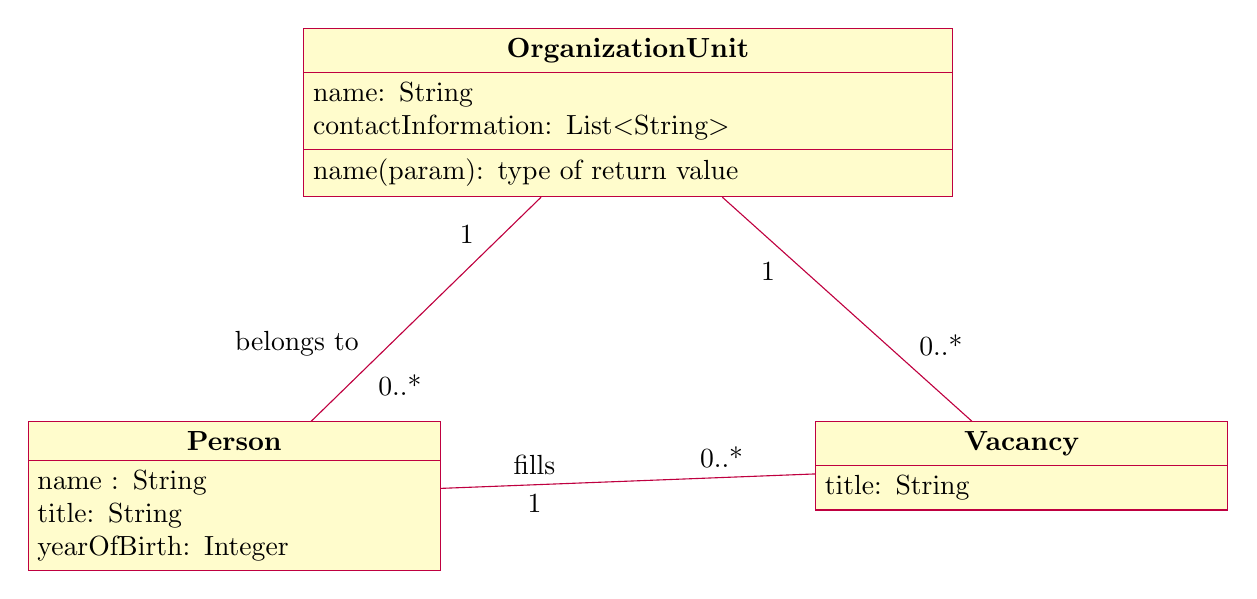
\begin{tikzpicture}   
    \begin{class}[text width=8 cm]{OrganizationUnit}{0,0}
      \attribute{name: String}
      \attribute{contactInformation: List$<$String$>$}
      \operation{name(param): type of return value}
    \end{class}
    \begin{class}{Person}{-5, -5}
      \attribute{name : String}
      \attribute{title: String}
      \attribute{yearOfBirth: Integer}
    \end{class}
    \begin{class}{Vacancy}{5, -5}
      \attribute{title: String}
    \end{class}
      
    \association{OrganizationUnit}{}{1}{Person}{0..*}{belongs to}  
    \association{OrganizationUnit}{}{1}{Vacancy}{0..*}{}  
    \association{Vacancy}{}{0..*}{Person}{1}{fills}
  \end{tikzpicture}
  \caption{AAA.}
\end{figure*}

\section{Structure}

\lipsum









\end{document}